% ============================================================
% Chaplygin sleigh -- schematic diagram (top-down view)
%
% Compiles standalone (crops tightly to the figure). To use inside
% an existing document, just copy the tikzpicture environment
% below into your file, and make sure your preamble has:
%   \usetikzlibrary{arrows.meta, angles, quotes, calc}
%
% Symbols:
%   O            blade (contact) point
%   C            center of mass
%   a = |OC|     distance from blade to center of mass
%   e1, e2       body-fixed frame at O; blade edge is along e1
%   theta        heading angle of the body w.r.t. the fixed X axis
%   v            velocity of O (nonholonomic constraint forces
%                v to lie along e1, i.e. v . e2 = 0)
%   omega        angular velocity of the body
%
% Tweak \sleighAngle, \bodyLen, \ocDist below to change the pose.
% ============================================================
\documentclass[tikz,border=4mm]{standalone}
\usepackage{amsmath}
\usetikzlibrary{arrows.meta, angles, quotes, calc}

\begin{document}
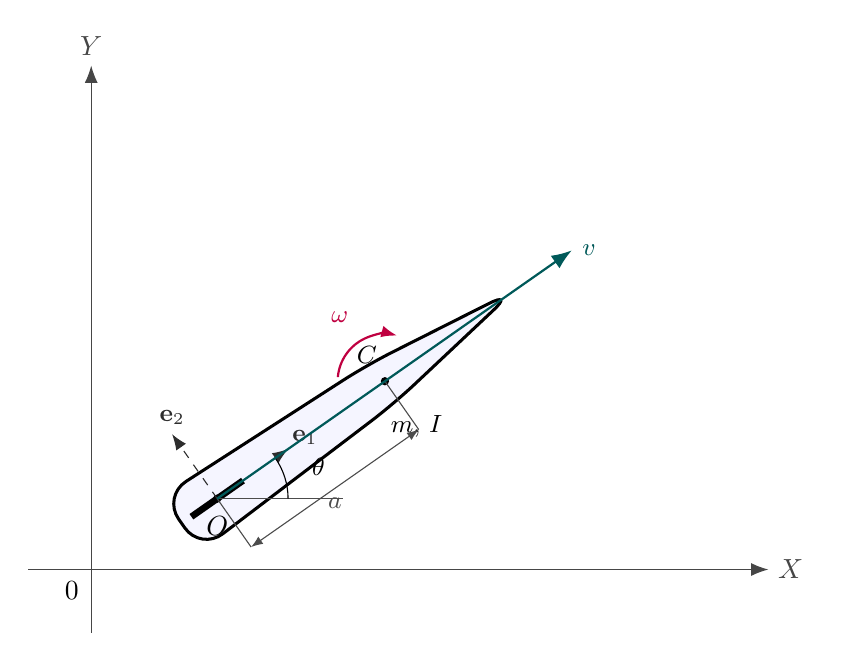
\begin{tikzpicture}[
    bodyline/.style ={line width=1.1pt, draw=black},
    axisline/.style ={-{Latex[length=2.2mm]}, gray!55!black, thin},
    framevec/.style ={-{Latex[length=2mm]}, gray!35!black, dashed},
    velvec/.style   ={-{Latex[length=2.6mm]}, thick, teal!70!black},
    omegavec/.style ={-{Latex[length=2mm]}, thick, purple},
    dimtick/.style  ={thin, black!70}
]

% ---------- pose parameters ----------
\def\sleighAngle{35}   % orientation of the body w.r.t. fixed X axis (deg)
\def\bodyLen{4.6}      % overall body length, O to nose
\def\ocDist{2.6}       % distance from blade point O to center of mass C

% ---------- fixed (lab) frame ----------
\draw[axisline] (-0.8,0) -- (8.6,0) node[right] {$X$};
\draw[axisline] (0,-0.8) -- (0,6.4) node[above] {$Y$};
\node[below left=1pt] at (0,0) {$0$};

% ---------- key points ----------
\coordinate (O)    at (1.6,0.9);
\coordinate (C)    at ($(O)+(\sleighAngle:\ocDist)$);
\coordinate (Nose) at ($(O)+(\sleighAngle:\bodyLen)$);
\coordinate (Xref) at ($(O)+(1.6,0)$);
\coordinate (E1ref) at ($(O)+(\sleighAngle:1.6)$);

% ---------- sleigh body (top-down silhouette) ----------
\draw[bodyline, rounded corners=10pt, fill=blue!4]
    ($(O)+(\sleighAngle:-0.55)+(\sleighAngle+90:0.42)$)
 -- ($(O)+(\sleighAngle:{0.55*\bodyLen})+(\sleighAngle+90:0.30)$)
 -- (Nose)
 -- ($(O)+(\sleighAngle:{0.55*\bodyLen})+(\sleighAngle+90:-0.30)$)
 -- ($(O)+(\sleighAngle:-0.55)+(\sleighAngle+90:-0.42)$)
 -- cycle;

% ---------- knife edge (blade) at O, aligned with e1 ----------
\draw[line width=2.4pt] ($(O)+(\sleighAngle:-0.4)$) -- ($(O)+(\sleighAngle:0.4)$);
\fill (O) circle (1.5pt);
\node[below=3pt] at (O) {$O$};

% ---------- center of mass ----------
\fill (C) circle (1.5pt);
\node[font=\small] at ($(C)+(\sleighAngle+90:0.4)$) {$C$};
\node[font=\small] at ($(C)+(\sleighAngle-90:0.7)$) {$m,\,I$};

% ---------- "a" dimension, offset below the body so it clears e1/v ----------
\coordinate (Oo) at ($(O)+(\sleighAngle-90:0.75)$);
\coordinate (Co) at ($(C)+(\sleighAngle-90:0.75)$);
\draw[dimtick] (O) -- (Oo);
\draw[dimtick] (C) -- (Co);
\draw[dimtick, {Latex[length=1.5mm]}-{Latex[length=1.5mm]}] (Oo) -- (Co)
    node[midway, below, font=\small] {$a$};

% ---------- body-fixed frame at O ----------
\draw[framevec] (O) -- ($(O)+(\sleighAngle:1.1)$)
    node[font=\small] [above right=-2pt] {$\mathbf{e}_1$};
\draw[framevec] (O) -- ($(O)+(\sleighAngle+90:1.0)$)
    node[font=\small, above] {$\mathbf{e}_2$};

% ---------- orientation angle theta ----------
\draw[dimtick] (O) -- (Xref);
\pic[draw, angle radius=9mm, angle eccentricity=1.5, "$\theta$"{font=\small}] {angle=Xref--O--E1ref};

% ---------- velocity of the blade point (constrained along e1) ----------
\draw[velvec] (O) -- ($(O)+(\sleighAngle:{\bodyLen+0.9})$) node[right, font=\small] {$v$};

% ---------- angular velocity (arc centered exactly at C) ----------
\draw[omegavec] ($(C)+({\sleighAngle+140}:0.6)$) arc ({\sleighAngle+140}:{\sleighAngle+40}:0.6);
\node[purple, font=\small] at ($(C)+(\sleighAngle+90:1.0)$) {$\omega$};

\end{tikzpicture}
\end{document}
